\section{Proposed Model and Methodology}\label{sec:methodology}

\subsection{Problem Formulation and Leakage Taxonomy}\label{sec:problem}

\subsubsection{Task Definition}

We formalize fraud detection on ERP and payment data as per-transaction
binary classification over a temporal, directed, attributed multigraph. Let
$\mathcal{V}$ denote the set of entities (accounts, vendors, G/L codes, or
customers, depending on the dataset) and let
$\mathcal{D} = \{e_1, e_2, \dots, e_N\}$ denote the transaction set, where
each transaction is a tuple
\[
e_i = (u_i, v_i, t_i, a_i, \mathbf{c}_i, y_i),
\]
with origin $u_i \in \mathcal{V}$, destination $v_i \in \mathcal{V}$,
timestamp $t_i \in \mathbb{R}$ (or an ordinal step/day index --
Section~\ref{sec:datasets} details each dataset's time axis), amount
$a_i \in \mathbb{R}_{>0}$, an auxiliary attribute vector $\mathbf{c}_i$
(transaction/document type, channel), and a binary label
$y_i \in \{0,1\}$ recording confirmed fraud. Transactions induce a directed
multigraph $G = (\mathcal{V}, \mathcal{D})$ that grows monotonically in
time; we write
\[
G_{\le T} \;=\; \bigl(\mathcal{V},\, \{\, e_j \in \mathcal{D} : t_j \le T \,\}\bigr)
\]
for the graph state immediately after every transaction up to and
including time $T$ has posted. The task is to fit a scoring function
$f_\theta : \mathbb{R}^d \to [0,1]$, applied to a feature vector
$x_i = \phi(e_i, G)$ extracted for each transaction, that approximates
$\Pr(y_i = 1 \mid x_i)$. Three feature families compose $x_i$ in this
project: ordinary transaction attributes ($a_i$, $\mathbf{c}_i$, calendar
features), structural/topology statistics computed from the graph (degree,
fan-in/out, lapping recurrence, cycle membership), and, where used, learned
temporal-graph embeddings (TGN) \cite{rossi2020temporal}. The graph
neural network literature has repeatedly reported structure-aware models
outperforming tabular baselines on financial fraud tasks
\cite{motie2024gnn,yuan2025survey}, almost always without an explicit audit
of the temporal-leakage failure modes formalized below; the dataset roster
in Section~\ref{sec:datasets} is chosen so that a fair, leakage-controlled
version of that comparison is possible across a genuine range of
structural richness. With the class prior $\Pr(y=1)$ ranging from roughly
0.12\% to 1.21\% across the real datasets studied here
(Table~\ref{tab:datasets}), we follow standard practice for severely
imbalanced classification \cite{bishop2006pattern} and evaluate with
threshold-independent ranking metrics (PR-AUC / average precision,
precision@$k$) rather than accuracy or a fixed decision threshold; the full
metric discussion and the modeling protocol built on it are given later in
this paper.

\subsubsection{Leakage-Free Feature Computation}

The single methodological requirement that dominates every other design
decision in this project is that $\phi$ must not use information
unavailable at the instant $e_i$ posts. We state this precisely.

\begin{quote}
\textbf{Definition (leakage-free feature map).} A feature map $\phi$ is
\emph{leakage-free} with respect to $\mathcal{D}$ if, for every transaction
$e_i \in \mathcal{D}$,
\[
\phi(e_i, G) \;=\; \phi(e_i, G_{\le t_i})
\]
for any $G \supseteq G_{\le t_i}$ -- that is, $\phi$'s output for $e_i$ is
invariant to which transactions with $t_j > t_i$ are or are not present in
the graph.
\end{quote}

Operationally we enforce this with a single streaming pass over
$\mathcal{D}$ in non-decreasing timestamp order: for each $e_i$, (1)
\emph{read} $x_i = \phi(e_i, G_{<t_i})$ against the graph state already
committed, then (2) \emph{insert} $e_i$'s edge and any derived state
(running counts, expanding means, open cycle candidates) before moving to
$e_{i+1}$. This read-then-insert ordering makes look-ahead structurally
impossible rather than merely policy-forbidden -- no code path exists
through which a later transaction's data can reach an earlier
transaction's feature vector. Two corollaries follow directly and are
enforced throughout the engine: (a) no statistic used in a feature
computation -- mean, standard deviation, per-account baseline, Benford
digit distribution -- may be computed once over the whole dataset; every
such statistic must be expanding or rolling over the past only, and (b)
when a structure (a cycle, a lapping sequence) is only detectable once its
final edge posts, its signal attaches to that \emph{completing}
transaction, never retroactively to the earlier transactions that merely
participated in it. Train/validation/test partitioning follows the same
discipline: splits are chronological -- train on the earliest period,
validate on the next, test on the latest -- never a randomly shuffled
$k$-fold, a protocol documented elsewhere to silently leak the future into
the past on time-evolving, dynamic fraud data \cite{jesus2022turning}.

\subsubsection{Leakage Taxonomy: Two Failure Modes in the Predecessor System}

An earlier iteration of this codebase reported headline metrics as strong
as $\mathrm{ROC\text{-}AUC} \approx 0.997$ on its flagship dataset and
concluded that graph topology was fraud detection's ``ultimate
differentiator.'' A pre-registration audit of that system's own artifacts
found the opposite: its topology detectors scored essentially 0.0 feature
importance, and every reported number was contaminated by two independent,
stacked leakage mechanisms. We name them Leak Class A and Leak Class B and
treat their elimination as this project's primary internal-validity
requirement.

\textbf{Leak Class A -- whole-graph feature computation.} The predecessor's
topology detectors ran once over the \emph{entire} graph, with no
$t_j \le t_i$ restriction anywhere, and each detected structure's signal
was written back to every member transaction, including its earliest ones
-- a cycle only observable once closed was nonetheless flagged on the edge
that opened it, directly violating the definition above. Two concrete
symptoms make the violation unambiguous: (i) a feature literally named
\texttt{time\_to\_next} -- the number of seconds until each account's
\emph{next} transaction -- ranked among the top five features by
importance; no detector can know the gap to a future transaction without
having already observed it. (ii) Every z-score / anomaly feature was
standardized against a whole-dataset mean and variance computed once, so a
transaction dated on day one was scored against a ``normal'' baseline that
included transactions from every later day, test period included.

\textbf{Leak Class B -- modeling-protocol leakage.} Four compounding,
confirmed malpractices were present in all five of the predecessor's
training scripts. (i) SMOTE oversampling and class-weighting were applied
\emph{simultaneously}, double-correcting for imbalance; because SMOTE's
$k$-nearest-neighbor interpolation was applied indiscriminately to
topology columns, it manufactured physically impossible points (a
synthetic transaction with, e.g., 0.4 of a closed cycle) that eased the
learned boundary without corresponding to any real fraud pattern. (ii)
Every reported metric used the library's default 0.5 decision threshold
(\texttt{.predict()}), never a threshold selected on held-out data --
meaningless when the positive class is 0.1--1.2\% of rows, since 0.5 is
not an operating point anyone chose. (iii) Cross-validation used
\texttt{StratifiedKFold} with shuffling and the timestamp column dropped
before fitting, so folds routinely trained on transactions dated after the
ones being scored, layering random-future leakage directly on top of Leak
A. (iv) Models were selected by F1 at that same fixed 0.5 threshold rather
than a threshold-independent, imbalance-appropriate ranking metric, which
rewards whichever leak-inflated configuration happens to look best at an
arbitrary cutoff rather than the one that generalizes.

\textbf{Why each invalidates the reported numbers.} Leak A inflates
apparent predictive power because the model is not learning what is
knowable at the moment an investigator would act -- it is learning the
correlation between a label and events that, by construction, occur after
the label's determining moment; the resulting metric is not an estimate of
deployable detection ability at all. Leak B compounds this at the
evaluation layer: synthetic minority points generated from a distribution
informed by the whole, undifferentiated dataset bias the decision boundary
toward the very examples later used to measure it; shuffled folds directly
violate the temporal ordering a fraud investigation depends on; and
selecting the ``best'' configuration by a metric computed under both prior
leaks means every design choice in the pipeline was made with implicit
knowledge of the answer it would later be graded on. Under datasets this
imbalanced -- as few as 19--25 confirmed fraud transactions in a single
evaluation split for SAP W\"urzburg (Section~\ref{sec:datasets}) -- even a
handful of leaked examples can move a headline metric by tens of points,
which is precisely the failure mode the leakage-free construction above,
and the ablation protocol built on it, are designed to make structurally
impossible rather than merely audited for after the fact.

%% FIGURE TODO: two-track timeline diagram. Top track: the correct
%% read-then-insert order -- for a transaction at time T, an arrow reads
%% features from graph state at T (pointing only left/backward in time),
%% then a second arrow commits/inserts the edge, moving strictly
%% left-to-right with no arrow ever pointing forward. Bottom track: the
%% predecessor system's Leak A pattern -- a completed-cycle icon at day 40
%% sends an arrow backward past day 40 to overwrite/attach to feature
%% values at day 3, visually contrasting causal vs. acausal attribution of
%% the same structure.
\begin{figure}[t]
  \centering
  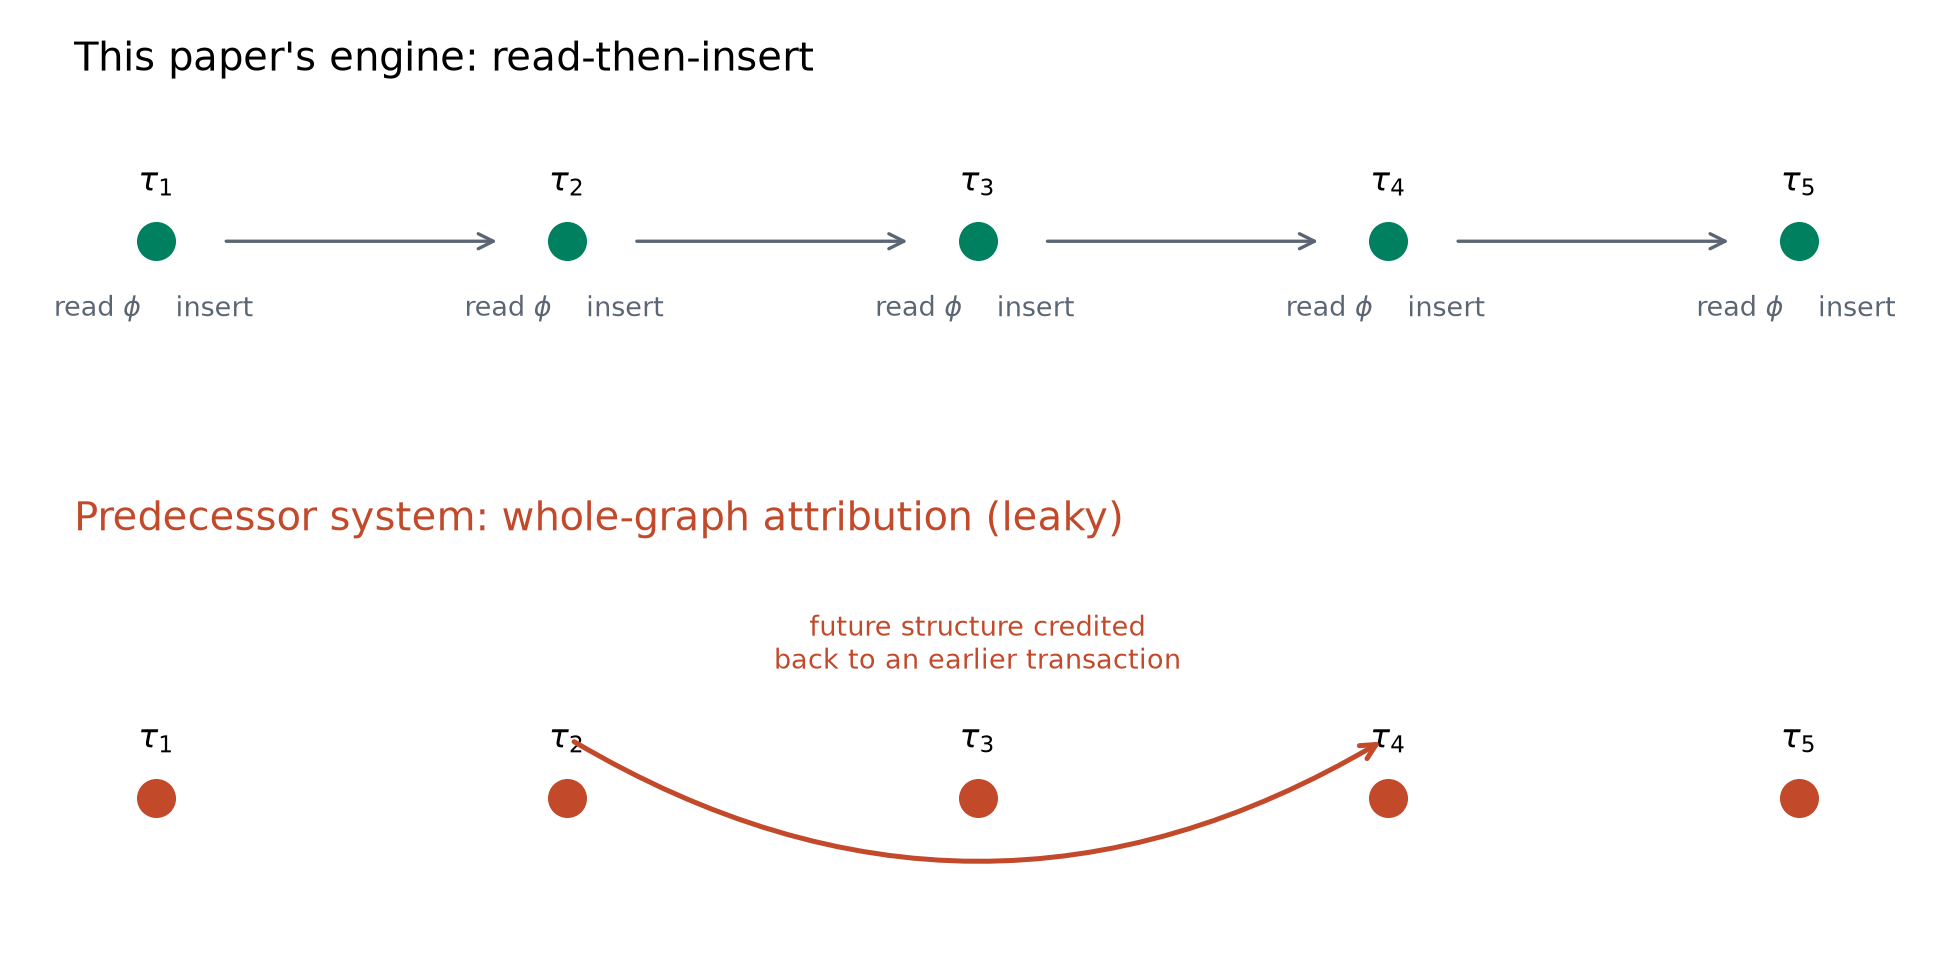
\includegraphics[width=\columnwidth]{figures/leakage_timeline.png}
  \caption{Read-then-insert feature computation (top) versus the
  predecessor system's whole-graph attribution (bottom), which credited a
  structure's signal back to transactions that occurred before the
  structure existed.}
  \label{fig:leakage_timeline}
\end{figure}

\subsection{Datasets}\label{sec:datasets}

\subsubsection{Overview and the Topology-Richness Spectrum}

Because the hypothesis under test is whether \emph{graph structure} carries
predictive signal beyond a strong tabular baseline, the dataset roster is
presented here as points along a topology-richness spectrum rather than as
an arbitrary convenience sample: from IBM AML, whose sender and receiver
identifiers occupy a near-unified account namespace supporting true
multi-hop cycles, down to PaySim, whose transaction graph is a near-forest
of one-off pairs. Table~\ref{tab:datasets} summarizes the four datasets
computationally profiled end-to-end in this study -- IBM AML, BankSim, SAP
W\"urzburg, and PaySim -- drawn from a single calibration pass over each
dataset's fully processed transaction table
(\texttt{calibration\_reference.json})
\cite{altman2023realistic,lopezrojas2014banksim,lopezrojas2016paysim}.
\emph{Kind} records each dataset's native graph topology: \texttt{Transfer}
(a directed account$\to$account graph, as in a payments network),
\texttt{Bipartite} (two structurally disjoint node classes with no
possibility of reciprocation or cycles), or \texttt{ERP ledger} (the
document-to-ledger-account bipartite structure specific to double-entry
ERP postings). \emph{NS Overlap} is the fraction of an account
namespace's senders that also appear as receivers -- the diagnostic this
project uses to certify whether same-entity cycles are even structurally
detectable; the predecessor system failed exactly this check by splitting
senders and receivers into disjoint node types, making a loop
$A\to B\to A$ structurally invisible regardless of how good its topology
engine was. \emph{Reciprocity} is the fraction of unique
(sender, receiver) pairs for which the reverse pair also transacted. Of
the four datasets in Table~\ref{tab:datasets}, only PaySim was profiled
without being modeled (Section~\ref{sec:paysim}).

\begin{table}[t]
\centering
\small
\caption{Graph-topology and scale summary of the four real datasets
computationally profiled in this study (source:
\texttt{calibration\_reference.json}). Amounts are in each dataset's
native units and are not comparable across datasets.}
\label{tab:datasets}
\resizebox{\columnwidth}{!}{%
\begin{tabular}{lccccccccc}
\toprule
Dataset & Kind & Fraud \% & $N_{\text{fraud}}$ & $N_{\text{txn}}$ & $N_{\text{acct}}$ & Amt.\ Med. & Benford MAD & NS Overlap & Recip. \\
\midrule
IBM AML       & Transfer    & 0.130 & 1{,}719 & 1{,}323{,}234 & 9{,}999       & 156.71      & 0.0758 & 0.9927 & 0.0446 \\
BankSim       & Bipartite   & 1.211 & 7{,}200 & 594{,}643     & 4{,}162       & 26.90       & 0.0319 & 0.0000 & 0.0000 \\
SAP W\"urzburg & ERP ledger & 0.124 & 248     & 200{,}629     & 59{,}883      & 1{,}975.80  & 0.0385 & 0.0000 & 0.0000 \\
PaySim        & Transfer    & 0.129 & 8{,}213 & 6{,}362{,}620 & 9{,}073{,}900 & 74{,}871.94 & 0.0142 & 0.0002 & 0.0000 \\
\bottomrule
\end{tabular}%
}
\end{table}

\subsubsection{IBM AML}

IBM AML is generated by the AMLSim multi-agent simulator and released as a
synthetic-but-structurally-realistic anti-money-laundering benchmark
\cite{altman2023realistic}. Its 1{,}323{,}234 transactions connect 9{,}999
accounts with a sender/receiver namespace overlap of 99.27\% -- the same
account IDs act as both senders and receivers almost everywhere, the
pre-condition this project treats as necessary for account-to-account
cycle detection to be structurally possible at all. Every transaction
carries the type \texttt{TRANSFER}; time is an integer day index over a
199-day span. At a fraud rate of 0.130\% (1{,}719 of 1{,}323{,}234), IBM
AML is this project's richest-structure testbed and the dataset on which
the topology hypothesis is given its best chance to succeed. It also
exhibits the sharpest amount anomaly of any dataset studied: fraud amounts
have median 10.60 and mean 9.76, against a full-population median of
156.71 and a mean of 115{,}988.18 (99th percentile 1{,}854{,}724.69) --
fraud in IBM AML clusters in a narrow, near-zero-value band while the
legitimate population is heavily right-skewed toward large transfers. We
read this as an artifact of the AMLSim generator's labeling convention
rather than a general property of laundering behavior, and it materially
shapes the ablation results discussed later in this paper: an
amount-based baseline that expects fraud to look large is directionally
wrong on this dataset, which is exactly what motivates evaluating an
amount-blind probe to isolate topology's contribution independent of this
artifact.

\subsubsection{BankSim}

BankSim is an agent-based simulation of a bank payment network built
specifically for fraud-detection research \cite{lopezrojas2014banksim}.
Its 594{,}643 transactions connect customer accounts (prefix \texttt{C})
to merchant accounts (prefix \texttt{M}) -- two structurally disjoint node
classes, so namespace overlap and pair reciprocity are both exactly 0.0
and no customer-to-customer or merchant-to-merchant cycle can exist by
construction. BankSim therefore serves this study as the sparse control:
any predictive lift topology features provide here must come from
bipartite-graph statistics (degree, fan-in/out, recurring near-equal
``lapping'' amounts) rather than from cycles, since cycles are
structurally unavailable. Its fraud rate, 1.211\% (7{,}200 of 594{,}643),
is the highest of the four real datasets, and its amounts are the smallest
in scale (median 26.90).

\subsubsection{SAP W\"urzburg}

SAP W\"urzburg is a real, publicly released SAP ERP transaction ledger and
is the only dataset in this study drawn from an actual production
accounting system rather than a simulator -- the setting continuous-
auditing research argues automated, always-on control monitoring should
target \cite{vasarhelyi2012acceptance}, and one that broader ERP-analytics
surveys still treat as an emerging rather than mature application of
machine learning \cite{jawad2024erp,mamakou2024postimplementation}. Its
graph is a document-to-account bipartite structure native to double-entry
bookkeeping: each posting document fans out to a small number of line
items (out-degree median 2.0, 99th percentile 10.0) that land on accounts,
a minority of which absorb a disproportionate share of postings (in-degree
99th percentile 43{,}706.7, maximum 46{,}554, against 59{,}883 distinct
account identifiers in total) -- a small core of heavily used ledger
accounts against a long tail of low-traffic counterparty accounts. With
only 248 confirmed frauds among 200{,}629 postings (0.124\%), SAP
W\"urzburg is this project's thinnest fraud signal by count, and, as the
ablation study reported later in this paper shows in full, the one real
dataset on which the full-model topology lift is measured
\emph{negative}. Two different SAP W\"urzburg train/validation/test
partitions appear elsewhere in this paper and should not be confused: the
chronological, partition-aware split used in the within-dataset ablation
study yields 120{,}411/40{,}137/40{,}139 rows
(\texttt{ablation.json}), while the multi-seed split used for final
champion-model selection yields 120{,}341/40{,}114/40{,}116 rows on the
same source file under a different, non-partition-aware split procedure
(\texttt{final\_champions.json}); both carry the same fraud counts by
split (204/19/25). We flag the discrepancy here so it does not appear
silently across two disconnected tables.

\subsubsection{IBM AML: Kaggle Reproduction Variant}

A second, independently downloaded instance of the IBM AML benchmark --
sourced directly from its Kaggle mirror rather than from the AMLSim-format
repository export behind the headline IBM AML numbers above -- was
processed during this build as a reproduction check on the deployed
\emph{online} scoring bundle, never as a source of headline results. The
two sources use different raw schemas (\texttt{TX\_ID}/
\texttt{SENDER\_ACCOUNT\_ID}-style AMLSim export versus the Kaggle
\texttt{HI-Small\_Trans.csv} layout) and are, in general, different
simulator draws; we report results under the separate label
\texttt{ibm\_aml\_kaggle} throughout, and none of its numbers are merged
into or averaged with \texttt{ibm\_aml}'s. For contrast -- though the two
are not directly comparable -- the offline champion model trained on the
primary \texttt{ibm\_aml} source, which includes TGN embeddings and, since
its TGN memory state is never persisted to disk, is not servable online at
all (a limitation discussed in full elsewhere in this paper), reaches a
saturated test PR-AUC of 1.00; that ceiling is itself uninformative given
the baseline's own 0.990 saturation (also discussed later in this paper).
\texttt{ibm\_aml\_kaggle}'s \emph{online} (ordinary+topology, non-TGN)
bundle -- the only kind of bundle this project ever serves in production
(\texttt{online\_bundles.json}) -- reaches a materially lower test PR-AUC
of 0.512 ($\pm$0.067 over three seeds, 26 features), consistent with both
the missing TGN component and the fact that the two \texttt{ibm\_aml}
variants are different simulator draws, not repeated measurements of the
same result.

\subsubsection{PaySim: Profiled, Not Modeled}\label{sec:paysim}

PaySim simulates a mobile-money transfer network at substantially larger
scale than any other dataset in this study -- 6{,}362{,}620 transactions
over 9{,}073{,}900 accounts \cite{lopezrojas2016paysim}, where almost
every transaction is the only time its particular (sender, receiver) pair
ever transacts (namespace overlap 0.0002, zero pair reciprocity, zero
repeat-pair transaction fraction). Its fraud rate, 0.129\% (8{,}213 of
6{,}362{,}620), sits in the same narrow band as IBM AML and SAP
W\"urzburg, but its graph is a near-forest at the opposite end of the
topology-richness spectrum from IBM AML: with essentially no repeated
edges between the same two accounts, most multi-hop structural detectors
(cycles, recurring lapping, degree accumulation) have little to attach to
before a transaction resolves. Consistent with this project's tiered
dataset plan, PaySim was carried through the ETL and topology-profiling
stages reported in Table~\ref{tab:datasets} but was never carried into
model training or the ablation study reported later in this paper; no
PR-AUC, precision@$k$, or lift number exists for it anywhere in this work,
and its row in Table~\ref{tab:datasets} should be read purely as a
structural reference point completing the spectrum, not as a modeling
result.

\subsubsection{The Synthetic Economy: synth\_erp}

\texttt{synth\_erp} is this project's own agent-based synthetic ERP
economy, spanning 39{,}256 accounts, generated deliberately \emph{after}
the real-data ablation protocol was designed, specifically to avoid the
circularity risk of injecting fraud in the exact shape a detector is built
to find -- a trap the predecessor system fell into by labeling injected
fraud literally \texttt{"Circular Payment"} or \texttt{"Lapping"}. Fraud is
instead generated from simulated criminal intent and evasion behavior, and
an independent adversarial leakage probe run against the resulting table
reports no exploitable single- or two-feature giveaway rule
(\texttt{leak\_flag: false}, \texttt{synth\_erp\_realism.json}); the worst
rule found, \texttt{tx\_type=transfer \& dest\_created\_midyear}, reaches
only 9.29\% precision at 43.75\% recall of fraud, a $19\times$ lift over
the 0.488\% base rate that is unremarkable next to a genuinely leaking
rule. At 1{,}148{,}503 transactions and a fraud rate of 0.488\% --
deliberately elevated above any real dataset's 0.124--1.211\% range to
keep minority-class training stable -- \texttt{synth\_erp} was built with
a near-unified account namespace (0.941 overlap) and the highest pair
reciprocity of any dataset in this study (0.136), by design, to give
topology detectors rich structure to find. Its amount distribution is, if
anything, \emph{too} clean relative to real data: a Benford MAD of 0.0047
is roughly three to sixteen times lower than any real dataset's
(0.0142--0.0758, Table~\ref{tab:datasets}) -- more compliant with
Benford's law than any of the messy real ledgers it is meant to
approximate, a known limitation of amount generation in synthetic
financial data that we surface rather than smooth over. Per the project's
own circularity safeguard, \texttt{synth\_erp} is used only for
training-time augmentation and stress-testing experiments, reported later
in this paper; it is never a source of this paper's headline ablation
claim, which is evaluated exclusively on the three real, independently
sourced datasets in Table~\ref{tab:datasets} that were carried into
modeling, plus SAP W\"urzburg's ERP-native structure specifically.

%% FIGURE TODO: scatter/bubble plot, x-axis = sender/receiver namespace
%% overlap (0 to 1), y-axis = pair reciprocity (0 to ~0.14), bubble area
%% = n_transactions (log scale), one labeled bubble per dataset (ibm_aml,
%% banksim, sap_wurzburg, paysim, synth_erp) -- visualizing the
%% topology-richness spectrum the roster is chosen to span, with ibm_aml
%% and synth_erp anchoring the structure-rich corner and banksim/
%% sap_wurzburg/paysim clustered at the structurally sparse origin.
\begin{figure}[t]
  \centering
  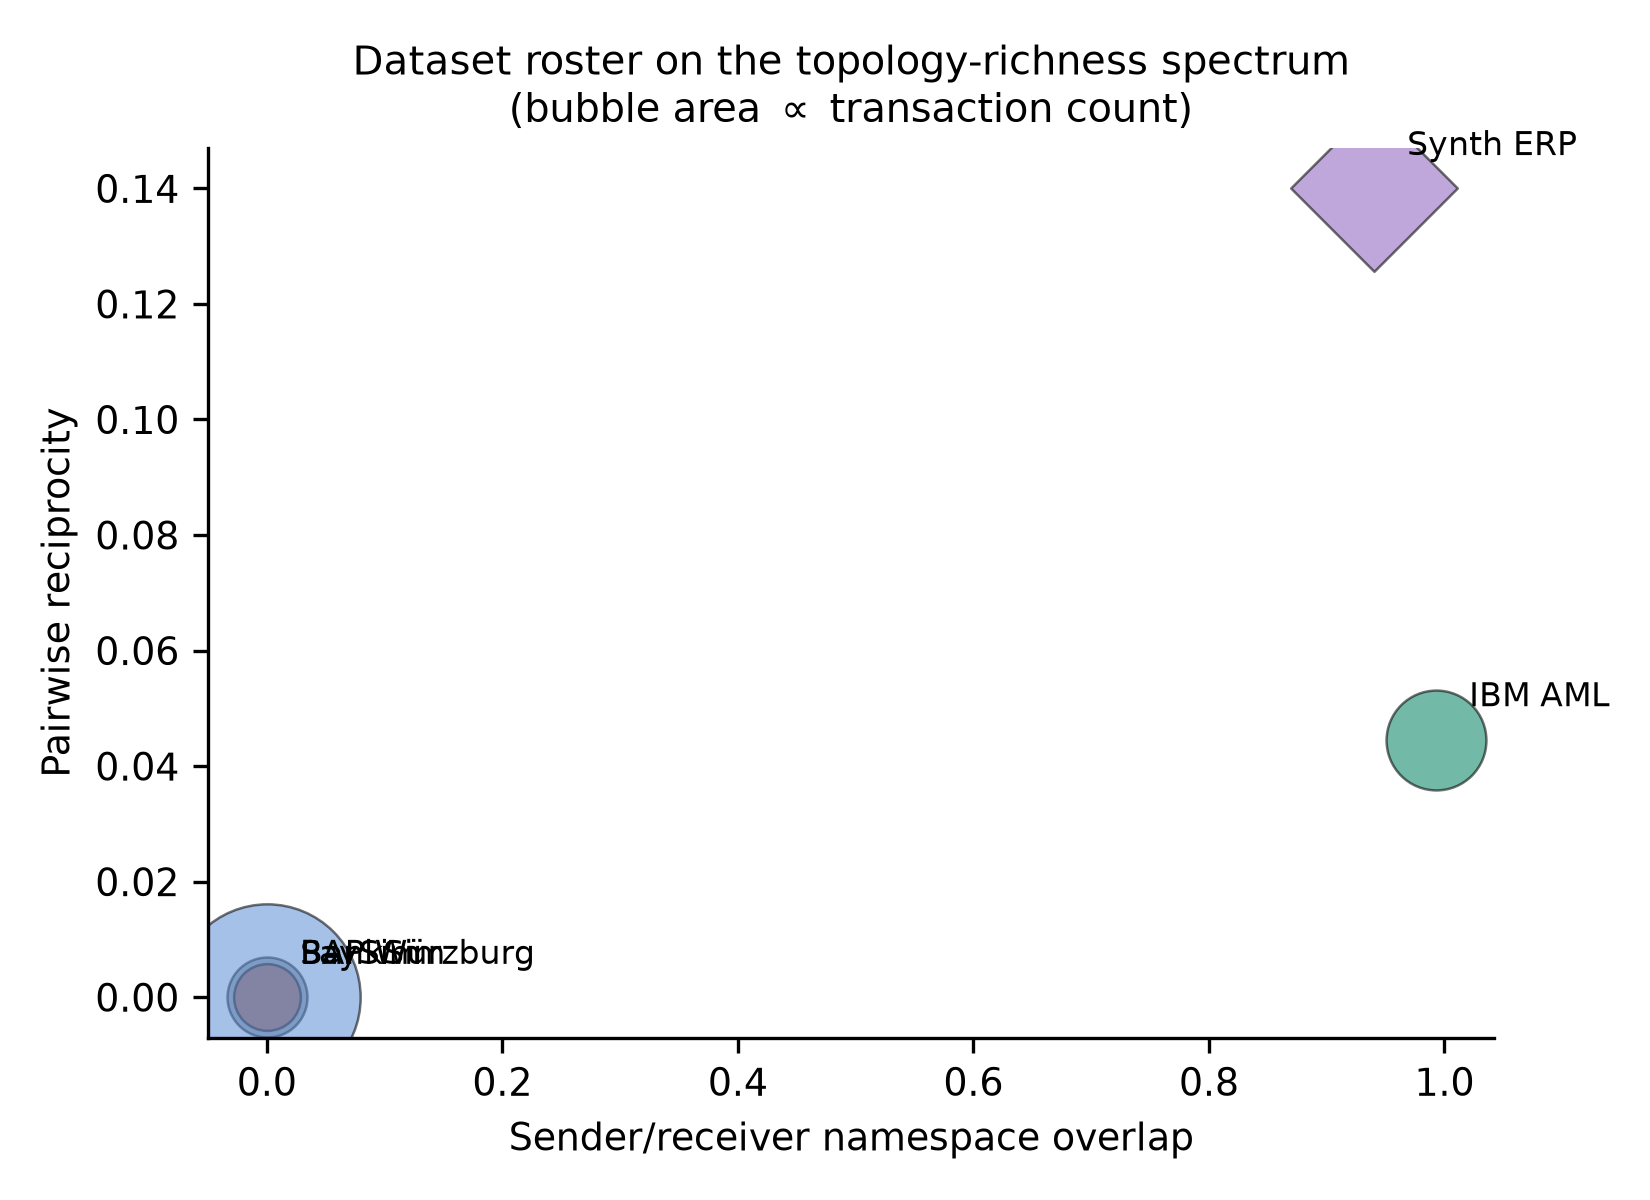
\includegraphics[width=\columnwidth]{figures/dataset_topology_spectrum.png}
  \caption{The five datasets positioned on the two structural axes this
  study uses to justify the roster: sender/receiver namespace overlap
  ($x$) and pair reciprocity ($y$), bubble area proportional to
  transaction count. IBM AML and \texttt{synth\_erp} anchor the
  structure-rich end; BankSim, SAP W\"urzburg, and PaySim anchor the
  structurally sparse end.}
  \label{fig:topology_spectrum}
\end{figure}

\subsection{Leakage-Free Temporal Topology Engine}\label{sec:engine}

A transaction does not reveal fraud in isolation; the same transfer can be
ordinary in one account context and the closing leg of a laundering cycle in
another. Graph-based fraud detection formalizes this by treating the ledger as
a network of who-paid-whom and searching for structural motifs — cycles,
fan-in collection points, rapid pass-through chains — that a row-wise view
cannot see~\cite{motie2024gnn,yuan2025survey,salih2021survey}. The difficulty
is computing such motifs \emph{as they would have been visible at the time},
without letting the completed, labeled dataset's hindsight leak into a
feature that is supposed to represent an auditor's knowledge at transaction
time. This section describes the streaming component of the Self-Auditing
Ledger that does this — the Temporal Topology Engine — and states, precisely
and with the project's own evidence, which of its thirteen output features
actually earn their keep.

The engine operates on the canonical edge list produced by ETL: one row per
transaction, with a source account, a destination account, a timestamp, an
amount, and (for training data) a fraud label. It is deliberately \emph{not}
a graph neural network and does not touch Neo4j; it is a single linear pass
over the sorted edge stream, maintained in pure Python/NumPy, that emits one
feature vector per transaction. Two data structures carry all state across
that pass: a trailing-window directed multigraph, \texttt{WindowGraph}, and a
per-account rolling amount memory, \texttt{LapMemory}. Both are described
below, followed by the thirteen features they jointly produce, the
structure/amount split used to keep the later ablation honest, and the
feature-importance result — including a null result the project does not
soften.

\subsubsection{The Leakage Invariant: Read, Then Insert}\label{sec:engine-invariant}

CLAUDE.md's rule 4 states the requirement in one sentence: a transaction's
features may depend only on transactions with \texttt{timestamp <=} its own.
The engine satisfies this not as a coding convention that a future edit could
quietly violate, but as a structural property of a single loop body. Edges
are pre-sorted by \texttt{(timestamp, transaction\_id)} — the ETL writes them
in this order with a stable sort, and the feature-assembly stage re-sorts
defensively if that invariant is ever violated upstream. The engine then
iterates \texttt{for i in range(n)} and, for transaction $i$, executes
exactly two kinds of statement in exactly one order:

\begin{enumerate}
  \item \textbf{Read.} Query \texttt{WindowGraph} for $i$'s fan-in, fan-out,
  destination in-degree, source out-degree, and (if $\mathrm{src}_i \neq
  \mathrm{dst}_i$) run the bounded cycle search; query \texttt{LapMemory} for
  the recurrence of $i$'s amount against each endpoint's rolling history.
  \item \textbf{Insert.} Only after every read above returns does the engine
  call \texttt{WindowGraph.add(t, u, v, amount)} and
  \texttt{LapMemory.record(\ldots)} for transaction $i$ itself.
\end{enumerate}

Because \texttt{add} for edge $j$ is called only during iteration $j$, and
iterations execute strictly in order $0, 1, \ldots, n-1$, the graph state
visible to iteration $i$'s reads is, by induction, exactly $\{j : j < i\}$
minus whatever \texttt{evict} has aged out — never a superset, and in
particular never anything from an iteration that has not yet run. No branch
of the loop calls \texttt{add} or \texttt{record} ahead of the paired reads
for the same $i$, and \texttt{evict} only removes edges whose timestamp falls
below \texttt{now - window}; it has no code path that admits an edge, only
ones that retire old ones. This is what we mean by \emph{leakage-free by
construction}: the claim does not rest on trusting that every caller remembers
to query before mutating, or on empirically observing no leak on the datasets
at hand — it follows from the fixed order of two statements inside one loop,
for any input that satisfies the pre-sort precondition. \texttt{LapMemory}
enforces the identical discipline: \texttt{recurrence(acct, amount)} is
always read before the same call site's \texttt{record(acct, amount,
counterparty)}. For SAP Würzburg, whose synthetic per-run time axis (encoded
as $\mathrm{run\_index}\times 10^{6} + \text{seconds-since-midnight}$) is not
a real cross-run chronology, both structures are additionally discarded and
rebuilt at every \texttt{run\_id} boundary, so a document in run 214 can never
borrow structural context assembled from a different, unrelated ledger run.

This constructive guarantee is checked, not merely asserted: an automated
leakage test (\texttt{topology.leakage\_test}) re-derives the same feature
table twice on real, built data — once truncated at the halfway point, and
once with every transaction \emph{after} the halfway point corrupted (shuffled
endpoints, amounts overwritten with an out-of-range sentinel) while
timestamps and row order are preserved — and asserts the first half's
features are byte-identical in both cases. This is deliberately redundant
with the constructive argument above: the constructive argument is the proof
that leakage is impossible for any input; the test is a regression guard that
would fail loudly if a future refactor moved a read after an insert. It has
run green throughout the build.

\subsubsection{The Trailing-Window Graph}\label{sec:engine-windowgraph}

\texttt{WindowGraph} holds a directed multigraph restricted to a trailing
time window $[\mathrm{now} - w, \mathrm{now}]$, where $w$ is a per-dataset
constant (7 days for IBM AML; 7 steps for BankSim, whose control role
requires \texttt{in\_cycle} to be identically zero everywhere since its
graph is customer$\to$merchant bipartite; 24 steps $=1$ day for PaySim; and
unbounded \emph{within} a run for SAP Würzburg, whose runs are short enough
that no window truncation is needed). Internally it keeps adjacency as
per-node dictionaries of neighbor multiplicities, so fan-in/fan-out (count of
\emph{distinct} counterparties) and weighted in-/out-degree (count
\emph{with} multiplicity) are both $O(1)$ lookups against the current
window state, and a deque of \texttt{(timestamp, u, v)} triples in arrival
order lets \texttt{evict(now)} pop expired edges from the front in amortized
$O(1)$ per evicted edge. The one non-trivial query is the cycle search: does
inserting $u \to v$ close a directed loop $v \rightsquigarrow u$ already
present in the window? This is answered by a breadth-first search from $v$
along existing out-edges, capped at \texttt{max\_cycle\_len}$-1$ hops (default
6) and a visited-node \texttt{search\_budget} (default 4{,}000); either bound
being hit returns "no cycle" rather than risk a false positive or an
unbounded cost on a dense hub account, so the detector is a conservative
under-approximation of the true cycle set, never an over-approximation. Each
directed pair also remembers the \texttt{(amount, timestamp)} of its most
recent in-window edge, which the cycle search folds together to report
amount conservation and timing tightness around the closed loop without a
second graph pass.

\subsubsection{Per-Account Lapping Memory}\label{sec:engine-lapmemory}

Lapping — using a new, similarly sized inflow to cover an earlier shortfall,
"robbing Peter to pay Paul" — is not naturally a graph-window feature: its
tell-tale recurrence can be separated by weeks or months, far longer than any
window size that keeps the cycle search cheap. \texttt{LapMemory} instead
keeps a fixed-length, \emph{count}-based rolling history of the last $k=25$
$(\text{amount}, \text{counterparty})$ pairs an account was involved in, in a
given role (incoming or outgoing) — two independent instances are kept per
account, one for each role. Because eviction is by count, not by elapsed
time, this memory spans exactly as much calendar time as the account's own
activity took to accumulate 25 transactions, so a dormant account that
reappears after a long gap is still compared against its own last known
pattern rather than an empty, window-truncated one. \texttt{recurrence(acct,
amount)} scans that account's stored history for entries within a relative
tolerance $\mathrm{tol}=1\%$ of the query amount and returns both the count of
matches and the number of \emph{distinct} counterparties among them. The
second number is what makes this a lapping detector rather than a
recurring-bill detector: one counterparty repeating the same payment every
month is ordinary billing, but several \emph{different} counterparties each
supplying a near-identical amount to the same account is the diversification
pattern lapping schemes exhibit. Reporting raw recurrence count alone would
fall into the same triviality trap as raw cycle membership (\S
\ref{sec:engine-finding}) — it fires constantly on legitimate recurring
payments — so counterparty diversity is carried as a co-equal, separate
feature rather than folded into a single scalar.

\subsubsection{The Thirteen Topology Features}\label{sec:engine-features}

Every transaction receives the same thirteen columns, grouped below by the
structure they measure; all are computed from the past-only graph/memory
state exactly as described above.

\textit{Cycle detectors (5).} \texttt{in\_cycle} is $1$ if the transaction
closes some directed loop within the window (a same-account self-payment
counts as a degenerate length-1 loop and is flagged directly, without a
search); \texttt{cycle\_length} is the edge count of the \emph{shortest} such
loop found, $0$ if none; \texttt{in\_cycle\_ge3} restricts this to loops of
length $\geq 3$, excluding both self-loops and simple reciprocal pairs
($A\to B\to A$), which are common and largely benign; \texttt{cycle\_amount\_ratio}
is $\min/\max$ of the amounts around the closed loop (including the closing
edge itself) — near $1$ means the money round-tripped with its value intact,
the discriminating signature of a wash trade rather than, say, a sale
followed by a small partial refund; \texttt{cycle\_time\_span} is the closing
transaction's timestamp minus the earliest edge on the loop — small values
mean the loop closed quickly, the "tightness" that separates a fast
laundering round-trip from an incidental, slow-forming one. Both are
\texttt{NaN} when no cycle closes, left as missing for the tree model rather
than imputed to zero.

\textit{Degree/fan detectors (4).} \texttt{fan\_in} and \texttt{fan\_out}
count, respectively, the number of \emph{distinct} accounts that have sent to
the destination account and the number of \emph{distinct} accounts the
source account has paid, within the window; \texttt{dest\_in\_degree} and
\texttt{src\_out\_degree} count the corresponding edges \emph{with}
multiplicity. The distinct/multiplicity pairing lets the model separate "many
different counterparties" (structuring, collection points) from "one
counterparty transacting repeatedly" (high degree, low fan) — the same
diversity-versus-repetition distinction the lapping features apply to
amounts.

\textit{Lapping detectors (4).} \texttt{lap\_in\_recur} and
\texttt{lap\_in\_payers} are \texttt{LapMemory.recurrence} evaluated against
the destination account's \emph{incoming}-amount history; \texttt{lap\_out\_recur}
and \texttt{lap\_out\_payees} the same against the source account's
\emph{outgoing}-amount history (\S\ref{sec:engine-lapmemory}).

\subsubsection{Structure vs.\ Amount: Why the Split Matters}\label{sec:engine-split}

Of the thirteen features, five are computed \emph{from transaction amounts}
— \texttt{cycle\_amount\_ratio} and all four lapping features — while the
remaining eight (\texttt{in\_cycle}, \texttt{cycle\_length},
\texttt{in\_cycle\_ge3}, \texttt{cycle\_time\_span}, \texttt{fan\_in},
\texttt{fan\_out}, \texttt{dest\_in\_degree}, \texttt{src\_out\_degree}) are
pure graph shape and never look at an amount value.
\texttt{cycle\_time\_span} is time-derived, not amount-derived, and is
counted with the structure group despite superficially "sounding" adjacent
to the amount features. The engine exposes this split (\texttt{topology\_structure\_cols}
vs.\ \texttt{topology\_amount\_cols} in the feature manifest) because the
ablation study's central probe — does topology help \emph{independent of the
amount signal}? — requires dropping every ordinary amount-derived tabular
feature (\texttt{log\_amount}, the expanding amount z-score, etc.)
\emph{and} every amount-derived topology feature together. Running an
"amount-blind" arm that strips the ordinary amount columns but leaves
\texttt{lap\_*} and \texttt{cycle\_amount\_ratio} in place would silently
re-admit the amount signal through the back door and overstate what pure
graph shape contributes. The structure-only arms in Table~\ref{tab:topology-importance}'s
source data (\texttt{no\_amount\_plus\_structure} in \texttt{paper/data/ablation.json})
are the clean version of this test; their interpretation is developed fully
in the ablation study.


\subsection{Modeling and Evaluation Protocol}\label{sec:protocol}

Every number reported in this paper and the next is produced by a single, shared training-and-evaluation harness applied identically to all four modeled datasets (BankSim, IBM~AML, SAP~W\"urzburg, and the in-house synth\_erp corpus). This section specifies that harness precisely enough to be reproduced: the learner and its fixed hyperparameter defaults, the two mutually exclusive imbalance mechanisms, the chronological splitting rule (including a partition-aware variant required by one dataset's own construction), the threshold-freezing procedure, the metric suite, and the attribution method. The harness is deliberately narrow — one function, one set of rules, applied the same way whether the feature set under test is a lean eight-column ordinary baseline or a ninety-nine-column champion bundle. Section~\ref{sec:ablation} then uses this exact protocol, unmodified, to answer the paper's central question.

\subsubsection{Model family: gradient-boosted trees, histogram method}
Every arm in this paper is an XGBoost classifier \cite{chen2016xgboost} with \texttt{tree\_method="hist"}, trained for up to 500 boosting rounds with early stopping after 40 rounds without validation-PR-AUC improvement. A single locked default configuration anchors every comparison: \texttt{max\_depth=6}, \texttt{learning\_rate=0.05}, \texttt{subsample=0.8}, \texttt{colsample\_bytree=0.8}, \texttt{min\_child\_weight=5}, \texttt{reg\_lambda=1.0}, \texttt{reg\_alpha=0.0}. Where a light random hyperparameter search (20 sampled configurations, scored on validation PR-AUC only) is run for a dataset's final champion, this default configuration is always included as candidate zero, so a tuned model can never underperform the untuned baseline on the selection metric it will be judged by. The search is automatically skipped when a split's validation-set fraud count is judged too small to support it without overfitting hyperparameters to a handful of positives — the guard that fires for SAP W\"urzburg (19 validation frauds), discussed further in \S\ref{sec:ablation-stats}.

Two other model families were deliberately not adopted as the classifier head, for reasons specific to this paper's ablation design rather than general performance claims. LightGBM~\cite{ke2017lightgbm} and Random Forest~\cite{breiman2001randomforests} are both viable gradient-boosted or bagged-tree alternatives to XGBoost and would very likely be TreeSHAP-compatible in the same way; XGBoost was retained throughout purely for harness consistency with this project's earlier committed artifacts, not because of a documented advantage over these alternatives, and re-running the ablation on either is named as future work rather than assumed unnecessary. Graph-native architectures — Kipf and Welling's GCN~\cite{kipf2017gcn}, Veli\v{c}kovi\'{c} et al.'s GAT~\cite{velickovic2018gat}, and Hamilton et al.'s GraphSAGE~\cite{hamilton2017graphsage} (see also Hamilton's
own textbook treatment of the broader graph-representation-learning field~\cite{hamilton2020graph})
— were considered and not adopted for a different, more consequential reason: none offers, out of the box, an attribution mechanism as cheap and exact as TreeSHAP's polynomial-time traversal of a fitted tree ensemble, and this paper's explainability requirement (every alert gets an exact, not sampled, per-feature attribution) is treated as a hard constraint on the model family, not a feature added after the fact. Lei et al.'s 2026 STC-MixHop~\cite{lei2026stcmixhop} is a recent graph-native architecture aimed at exactly this paper's problem setting (non-stationary transaction fraud), and its own reported finding — that a graph-native model struggles to outperform a tabular baseline precisely where node attributes already carry strong signal — is consistent with, and independently motivates, this paper's decision to route learned graph signal (via TGN) into TreeSHAP-explainable tabular features rather than deploy a graph-native model end to end.

\subsubsection{One imbalance mechanism, never two}
Fraud rates in the four datasets range from roughly 0.1\% to 1.2\% of rows. The harness offers exactly two ways to counteract this, selected per run and recorded in every saved artifact, and never combined: (i) \emph{class weighting}, XGBoost's native \texttt{scale\_pos\_weight} set to the train-split negative-to-positive ratio, and (ii) an \emph{alpha-free focal-loss} objective \cite{lin2017focal}, implemented as a custom XGBoost objective with a closed-form gradient and a central-finite-difference Hessian, trained with \texttt{scale\_pos\_weight=1.0}. The focal variant is deliberately \emph{unweighted} (symmetric, no per-class $\alpha$ term): the common alpha-balanced formulation of focal loss secretly reintroduces a class-prior weight, which would silently stack a second imbalance mechanism on top of the first — precisely the failure mode this protocol is built to exclude. Because a focal objective returns a raw margin rather than a probability, every downstream consumer (threshold tuning, PR-AUC, TreeSHAP) is written to accept either representation, applying a sigmoid only where a probability is actually required. Synthetic minority oversampling (SMOTE) is excluded from the harness entirely, on the grounds that an interpolated point between two topology vectors — half a cycle, a fractional fan-in count — has no physical meaning in a transaction graph.

Which mechanism wins is decided the same way as any other hyperparameter: on validation-split PR-AUC, never on the test split. Per \texttt{final\_champions.json}, focal loss wins the selection on three of the four datasets — BankSim (validation PR-AUC mean $0.9515$ vs.\ $0.94891$ for class weighting), SAP W\"urzburg ($0.35619$ vs.\ $0.28875$, though this particular selection is separately flagged \texttt{reliable:\ false} owing to the small-sample guard above), and synth\_erp ($0.85066$ vs.\ $0.84866$). IBM~AML is the exception, and an instructive one: both mechanisms reach a validation PR-AUC of exactly $1.0$ with zero variance across three seeds, so the "winner" (class weighting, by tie-break) is not really a comparison at all — an early symptom of the baseline-saturation story developed in \S\ref{sec:ablation}.

\subsubsection{Chronological splitting, including a partition-aware variant}
Every split is a 60/20/20 train/validation/test partition by transaction timestamp, and rows are never shuffled: the training set is defined as the earliest 60\% of transactions by time, validation the next 20\%, and test the final, strictly future 20\%. For most datasets this is a single global quantile cut on the timestamp axis. SAP W\"urzburg is the exception: its raw export orders postings by \texttt{run\_id} (audit run), and each run is internally fraud-first-then-clean, so a global time cut would strand an entire zero-fraud run inside the validation split. The harness therefore applies a \emph{partition-aware} variant for this dataset — the same 60/20/20 chronological rule, but computed independently within each \texttt{run\_id} and concatenated, so every run contributes its own early rows to train and its own late rows to test. This is still a strictly chronological, never-shuffled split; only the unit over which the time cut is computed changes.

Two independent partition-aware splits of SAP W\"urzburg appear in this project's own committed artifacts, and they differ by a small margin that we flag rather than silently reconcile. The ablation run (\texttt{ablation.json}) reports train/val/test sizes of $120{,}411$/$40{,}137$/$40{,}139$; the later final-champion run (\texttt{final\_champions.json}) reports $120{,}341$/$40{,}114$/$40{,}116$ — a difference of 116 rows, or about 0.06\% of the dataset. Both runs use the identical partition-aware algorithm described above, so the discrepancy is not a change in splitting logic; it most plausibly reflects a small difference in row count between two separate ETL/feature-build passes of the same source file. We did not further trace its exact origin. Every SAP W\"urzburg figure in this paper is therefore attributed to the specific source file it was read from, and the two split-size counts should not be added, averaged, or treated as interchangeable.

\subsubsection{Threshold tuning: frozen before the test set is touched}
XGBoost outputs a continuous score; converting it into a binary alert requires a cutoff, and an arbitrary $0.5$ is never used. Instead, the harness scans the validation-set precision--recall curve and selects the threshold that maximizes F1 on validation data alone. That threshold is then frozen and applied, unmodified, to the held-out test split — the test set never participates in threshold selection. In practice the chosen threshold varies considerably by feature set even within one dataset (for BankSim, $0.9673$ for the ordinary baseline vs.\ $0.9549$ for the topology-augmented model; \texttt{ablation.json}), underscoring why a single fixed cutoff across models would confound feature-set comparisons with cutoff artifacts.

\subsubsection{Primary and operational metrics}
PR-AUC (average precision) is the primary metric throughout this paper and the sole metric used for model and mechanism selection; it is never selected on F1-at-a-fixed-threshold, which would hide the cutoff problem the previous subsection exists to solve. ROC-AUC is reported alongside it but never relied upon: on data this skewed (fraud rates of 0.1--1.2\%), ROC-AUC is inflated by the overwhelming volume of easy true negatives and routinely exceeds 0.99 even for models with weak operational precision (Table~\ref{tab:ablation-arms}, SAP W\"urzburg's baseline arm: ROC-AUC $0.991$ against a PR-AUC of only $0.155$). This choice follows a well-established methodological literature rather than project-local intuition: Provost et al.~\cite{provost1998case} first argue against single-number accuracy estimation for comparing induction algorithms on skewed data, Davis and Goadrich~\cite{davis2006relationship} formalize the precision-recall/ROC relationship and show a curve dominant in ROC space need not be dominant in PR space, and Saito and Rehmsmeier~\cite{saito2015prauc} demonstrate directly that the PR plot is more informative than the ROC plot specifically when evaluating binary classifiers on imbalanced data of the kind studied throughout this paper. Because an audit team reviews a bounded daily list of alerts rather than a probability distribution \cite{vasarhelyi2012acceptance}, every evaluation also reports precision@$k$ and recall@$k$ for $k \in \{50, 100, 500, 1000\}$ — of the top-$k$ highest-scored transactions, what fraction are confirmed fraud, and what fraction of all fraud that budget would catch. F1 at the frozen threshold is reported for completeness but, as noted, is never a selection criterion.

\subsubsection{Attribution: exact TreeSHAP in margin space}
Every reported feature attribution is computed via XGBoost's native \texttt{pred\_contribs} interface rather than a sampling-based SHAP approximation. With \texttt{pred\_contribs=True}, the booster runs the exact TreeSHAP recursion \cite{lundberg2017unified,lundberg2020local} — algorithmically identical to the \texttt{shap} package's \texttt{TreeExplainer} for tree ensembles — as a pure traversal of the fitted trees, returning one signed contribution per feature per row plus a base value, additive in margin (log-odds) space. This is exact, not approximate, and its cost is a fixed function of tree structure rather than a sampling budget. It is also, crucially, agnostic to which of the two imbalance mechanisms trained the model: because a focal-loss booster is still an ordinary ensemble of regression trees whose leaves were fit against a focal gradient, the same margin-space traversal applies unchanged, with only the final sigmoid step (used only where a probability is required, e.g.\ threshold comparisons) built to know which mechanism produced the raw score. This gives every model in this paper's evaluation suite — baseline, topology-augmented, and the final TGN-plus-topology champion alike — an exact, common explanation mechanism, discussed further in the explainability sections that follow. This is not merely a technical convenience: Faccia~\cite{faccia2026xaiauditing} and Uddin and Aziz~\cite{uddin2026shapley} both report, from independent 2026 studies of regulatory-facing fraud-detection auditing, that exact tree-native attribution is materially more stable and more defensible under audit scrutiny than either a sampled SHAP approximation or a post-hoc explanation layered onto a deep architecture — the same practical constraint that rules out an end-to-end neural classifier for this paper's production console regardless of its raw predictive accuracy.

\subsection{The Ablation: Experimental Design}\label{sec:ablation-design}

The protocol of \S\ref{sec:protocol} exists to answer one question honestly: \emph{do graph-topology features add predictive value over a strong ordinary-transaction baseline, measured without leakage?} This section reports that answer as a seven-arm ablation run identically, with identical splits, model family, and imbalance-mechanism selection, on each of the four modeled datasets. We commit, per the project's own methodology rules, to reporting the result exactly as measured — including where it is negative, where it is uninformative, and where it rests on too few positive examples to trust.

\subsubsection{The seven-arm decomposition}
A naive ablation — ordinary features alone vs.\ ordinary-plus-topology — is not sufficient here for two reasons uncovered during this project's own earlier probing. First, on a dataset whose ordinary-only baseline is already close to saturated (IBM~AML: baseline PR-AUC $0.990$), a marginal comparison against the full model has almost no headroom left to measure, whatever the true value of topology. Second, several of the project's topology detectors are not, in fact, amount-blind: the lapping detectors (\texttt{lap\_in\_payers}, \texttt{lap\_in\_recur}, \texttt{lap\_out\_payees}, \texttt{lap\_out\_recur}) and the cycle amount-conservation ratio (\texttt{cycle\_amount\_ratio}) are derived in part from transaction amounts, so a topology arm that includes them can re-smuggle the amount signal into what is presented as a "structural" result. Of the thirteen topology features produced by the engine, the feature manifests confirm this split is exact and identical across all four datasets: eight are pure structure (\texttt{in\_cycle}, \texttt{cycle\_length}, \texttt{in\_cycle\_ge3}, \texttt{cycle\_time\_span}, \texttt{fan\_in}, \texttt{fan\_out}, \texttt{dest\_in\_degree}, \texttt{src\_out\_degree}), and five are amount-derived (the four lapping features plus \texttt{cycle\_amount\_ratio}).

The ablation therefore trains seven arms per dataset, all under the identical protocol of \S\ref{sec:protocol}: (1) \textbf{Baseline} — ordinary transaction features only; (2) \textbf{+Topology} — baseline plus all thirteen topology features, amount-derived ones included; (3) \textbf{+Structure} — baseline plus only the eight pure-structure features; (4) \textbf{Amount-blind baseline} — the ordinary feature set with every amount-derived column (log-amount, amount z-scores, prior amount means, \ldots) removed; (5) \textbf{Amount-blind~+~Topology}; (6) \textbf{Amount-blind~+~Structure}; and (7) \textbf{Topology-only} — the thirteen topology features with no ordinary features at all. Only arms (1) and (2) are persisted as deployable model artifacts; the remaining five exist purely to decompose \emph{why} any observed lift occurs.

From these seven arms, four scalar lift statistics are computed on the test split, each isolating a different confound:
\begin{itemize}
  \item \textbf{marginal\_topology\_lift} = PR-AUC(+Topology) $-$ PR-AUC(Baseline) — the headline number, but contaminated by amount-derived topology on a full-featured model;
  \item \textbf{marginal\_structure\_lift} = PR-AUC(+Structure) $-$ PR-AUC(Baseline) — the honest full-model claim, restricted to pure structure;
  \item \textbf{amount\_blind\_topology\_lift} = PR-AUC(Amount-blind+Topology) $-$ PR-AUC(Amount-blind baseline) — removes the amount confound from the baseline, but still contaminated because the topology arm itself contains amount-derived columns;
  \item \textbf{amount\_blind\_structure\_lift} = PR-AUC(Amount-blind+Structure) $-$ PR-AUC(Amount-blind baseline) — the \emph{clean} test: no amount information anywhere, on either side of the comparison.
\end{itemize}
Only the last of these four is free of both confounds simultaneously, and it is the number we treat as the decisive evidence for or against the paper's thesis on each dataset.

\subsection{A Calibrated Synthetic ERP Economy: Generator Design}\label{sec:synthetic}

The four real datasets used elsewhere in this paper give us, at best, a few
thousand labeled fraud rows each, concentrated in typologies each simulator's
original authors happened to encode. To probe typologies we do not observe at
scale in any single real ledger, and to obtain a dataset that is simultaneously
account-to-account (so that cycles are structurally possible), ERP-flavored
(payables, payroll, receivables), and large enough in fraud count to support
per-typology analysis, we built \texttt{synth\_erp}: an agent-based simulation
of a 40-company economy running for 365 simulated days over $\sim$39k accounts,
producing 1{,}148{,}503 transactions of which 5{,}609 are labeled fraud
(a 0.4884\% rate). This section documents how the generator was designed to
resist the one failure mode that would make it useless for our purposes, what
an independent realism audit against the four real datasets found — including
where the synthetic economy does \emph{not} match reality — and what a direct
adversarial probe for cheap tabular leaks and a downstream training-transfer
experiment revealed. Throughout, we hold \texttt{synth\_erp} to the same
evidentiary standard as the real datasets: numbers are reported whether or not
they are flattering, because the entire purpose of this exercise is to know
which sanctioned use cases actually survive scrutiny.

\subsubsection{Design Philosophy: The Circularity Trap}
\label{sec:synthetic-trap}

A synthetic fraud generator built by the same team that builds the fraud
\emph{detector} is exposed to an obvious failure mode: if the generator's
authors hand-encode fraud as ``insert a 3-hop cycle'' or ``make the receiver's
in-degree spike,'' a topology engine built by the same authors will of course
find it — not because graph structure is informative about fraud in general,
but because the two pieces of code were written to fit each other. Grading a
detector against a generator that shares its assumptions proves nothing about
the real world; it is closer to checking that a lock opens with its own key.
\texttt{synth\_erp} was designed against this failure mode by a single binding
rule, carried in this project's own methodology documentation: fraud is
injected as \emph{goal-driven behavior with evasion}, never as a
detector-shaped pattern. The fraud-generation code imports nothing from the
topology-feature codebase and references no detector's internals; every
typology is written as an agent pursuing a criminal objective (skim a
receivable, drain a payables account, collect from recruited mules) under
realistic constraints (approval thresholds, banking hours, evasion timing),
and any cycle, fan-in, or amount-recurrence a detector later measures is a
\emph{consequence} of that behavior, not its specification. The benign
population mirrors this discipline: ordinary commerce is allowed to produce
the same raw ingredients fraud produces — busy retailers with heavy fan-in,
payroll batches that resemble fan-out bursts, subscription billing that
recurs at a near-equal amount, refunds that close reciprocal pairs, multi-hop
circulation as salaries fund purchases that fund vendors — since a background
in which only fraud has structure would reintroduce the same shortcut through
the back door. Sec.~\ref{sec:synthetic-emergence} reports just how modestly
enriched the fraud-typology structural traces actually are once this
constraint is honored — a dataset engineered to make cycles trivially
separable would show the opposite pattern.

\subsubsection{Generator Architecture, Scale, and Transaction Composition}

\texttt{synth\_erp} follows the same broad methodology family as two of the
real datasets used elsewhere in this paper — an agent-based simulation
calibrated against measured real-world statistics rather than a purely
hand-tuned generator, the approach behind BankSim~\cite{lopezrojas2014banksim},
PaySim~\cite{lopezrojas2016paysim}, and the AMLSim lineage behind
\texttt{ibm\_aml}~\cite{altman2023realistic}. This is a deliberately different
generative paradigm from the deep generative models increasingly used
elsewhere in the fraud-synthesis literature — GAN-based transaction
synthesis~\cite{wang2023syntheticgan,zhu2024gansfraud} traces back to
Goodfellow et al.'s original adversarial framework~\cite{goodfellow2014gan},
and a variational alternative traces to Kingma and Welling's VAE~\cite{kingma2014vae}.
Both families belong to the broader deep generative modeling literature~\cite{goodfellow2016deep}
and learn a data distribution from observed examples and sample
from it; an agent-based simulator instead specifies \emph{behavior} (an
account's transaction habits, a fraud typology's goal and evasion strategy)
and lets structure emerge from that behavior's interaction with other
agents. We chose the agent-based approach specifically because it is the
only one of the two that supports this section's non-circularity
requirement (\S\ref{sec:synthetic-trap}): a GAN or VAE trained to reproduce
the statistical signature of labeled fraud would, definitionally, learn
whatever shape the training examples already have, which is the exact
grading-your-own-homework risk this generator is built to avoid. The simulated economy comprises
40 companies operating alongside their customers, vendors, and employees,
generating seven ordinary transaction flows
(\texttt{sale}, \texttt{vendor\_payment}, \texttt{payroll}, \texttt{transfer},
\texttt{refund}, \texttt{reimbursement}, \texttt{recurring\_bill}) over a full
simulated year. Table~\ref{tab:synth-flows} gives the exact per-flow
transaction counts, read directly from the same adversarial tabular-leak audit
discussed in Sec.~\ref{sec:synthetic-leakprobe} (the per-\texttt{tx\_type}
support counts there sum exactly to the dataset total, confirming the two are
consistent measurements of the same underlying table). Retail \texttt{sale}
traffic dominates by volume (66.2\%), with the ERP-specific payables rail
(\texttt{vendor\_payment}, 18.1\%) the second-largest flow — a composition
deliberately closer to an operating company's ledger than to a pure
consumer-payments simulator.

\begin{table}[t]
\centering
\small
\caption{Transaction volume by flow type, \texttt{synth\_erp} (all 1{,}148{,}503 rows, fraud and benign combined). Source: \texttt{paper/data/synth\_erp\_realism.json}, \texttt{tabular\_leak\_probe.rules} per-\texttt{tx\_type} support.}
\label{tab:synth-flows}
\begin{tabular}{@{}lrr@{}}
\toprule
Flow (\texttt{tx\_type}) & Count & Share \\
\midrule
\texttt{sale}            & 760{,}558 & 66.23\% \\
\texttt{vendor\_payment}  & 208{,}155 & 18.13\% \\
\texttt{transfer}         &  94{,}781 &  8.25\% \\
\texttt{payroll}          &  49{,}240 &  4.29\% \\
\texttt{refund}           &  18{,}396 &  1.60\% \\
\texttt{reimbursement}    &  12{,}236 &  1.07\% \\
\texttt{recurring\_bill}  &   5{,}137 &  0.45\% \\
\midrule
Total                     & 1{,}148{,}503 & 100.00\% \\
\bottomrule
\end{tabular}
\end{table}

At the account/graph level, the simulated economy is dense and repeat-heavy:
39{,}256 accounts transact across 251{,}192 unique sender--receiver pairs,
with 85.86\% of transactions occurring between a pair that has transacted
before (\texttt{repeat\_pair\_txn\_frac} = 0.8586) and 94.1\% of accounts
appearing on both the sending and receiving side of at least one transaction
(\texttt{namespace\_overlap} = 0.941) — i.e., this is deliberately \emph{not}
a bipartite consumer-to-merchant graph, since ERP economies circulate money
(salaries fund purchases, purchases fund vendors, vendors pay employees) in a
way that pure-payments simulators structurally cannot. Degree is heavy-tailed
in both directions: median out-degree 18 (p99 = 83, max = 20{,}838) and
median in-degree 4 (p99 $\approx$ 128, max = 194{,}265), driven by a small
number of high-volume retailers and payroll-issuing companies. Activity is
temporally realistic without being explicitly targeted at any metric: 79.06\%
of transactions fall in business hours and 17.31\% on weekends, at a mean of
3{,}146.6 transactions/day (p99 = 5{,}308.3) sustained across all 365 simulated
days — timestamped to the second, a finer time axis than any of the four real
datasets in our roster provide.

\subsubsection{Five Fraud Typologies as Emergent Behavior}
\label{sec:synthetic-emergence}

Fraud is injected as five occupational-fraud typologies, each defined by an
actor's goal and evasion strategy rather than by a target graph shape:
\texttt{laundering\_cycle} (embezzled funds layered through a ring of shells
and, in most scenarios, cycled back toward the entry account), \texttt{mule\_fanin}
(scam proceeds collected from many recruited mule accounts into one
collector), \texttt{lapping} (a diverted receivable covered days later by the
next customer's payment), \texttt{invoice\_kickback} (a colluding vendor
overbills and returns a cut to an insider), and \texttt{larceny} (direct
insider diversion of funds, disguised as vendor or reimbursement traffic). The
resulting typology counts are 1{,}442 (\texttt{laundering\_cycle}), 2{,}327
(\texttt{mule\_fanin}), 760 (\texttt{lapping}), 625 (\texttt{invoice\_kickback}),
and 455 (\texttt{larceny}) labeled rows, summing to the reported 5{,}609
fraud transactions.

Because these behaviors are never specified in terms of detector features, the
honest question is whether they leave structural traces at all, and at what
rate. The benign background already contains a nontrivial rate of graph
cycles — 5.761\% of benign transactions close a cycle in the observed window,
with 99th-percentile benign fan-in reaching 4{,}197 distinct senders (busy
retailers and payroll hubs) — so cyclicity and fan-in are not, by
construction, fraud-exclusive signals. Against that background,
\texttt{laundering\_cycle} transactions close a cycle 18.45\% of the time (all
at length $\geq 3$), a $3.2\times$ enrichment over the 5.761\% benign base
rate — real, but far from deterministic, consistent with a design in which
60\% of rings loop back to their entry account and 40\% exit linearly, and in
which the streaming, look-ahead-free topology engine's window will miss some
closures entirely. \texttt{mule\_fanin} collectors show a 90th-percentile
in-window fan-in of only 8 distinct senders — far below the benign
99th-percentile of 4{,}197 — so a raw fan-in threshold offers no free
discrimination there either. \texttt{lapping} shows the weakest structural
footprint of the five: its amount-recurrence measure
(\texttt{lap\_in\_recur}) averages 0.06, swamped by a benign population
dominated by genuinely recurring payroll and subscription billing. We flag
this pattern explicitly because it foreshadows a headline finding developed
later in this paper (Sec.~\ref{sec:ablation}): engineered cycle-shaped
features carry a surprisingly small share of the detectable signal on real
data, and this section shows that is not an artifact of an unrealistic
generator — even in a dataset whose typologies are explicitly designed to
produce cycles and fan-in, those structural traces are only modestly
enriched over an already-active benign background, not deterministic
markers.

\subsection{Explainable Audit Alerts: Methodology}\label{sec:explain}

A probability score by itself is not evidence an auditor can act on.
Opening or closing an investigation requires knowing \emph{why} a
transaction scored high and \emph{what}, concretely, is suspicious about
it -- ideally with a guarantee that the latter is not a plausible-sounding
story invented after the fact. Post-hoc graph-neural-network explainers
typically supply only an approximate, model-external account of that kind
\cite{wang2023reinforced}. The console instead attaches every alert a
fixed, two-layer explanation, both layers computed once per alert directly
from the persisted scoring bundle and the canonical transaction stream
(\texttt{src/modeling/alerts.py}): (1) exact per-feature attribution of the
score, tagged by feature family and glossed in plain English, and (2) graph
evidence obtained by literally replaying the transaction stream to the
alert's exact position in time, so that what the auditor is shown is
provably consistent with what the model saw rather than a post-hoc
rationalization. Every alert below is generated from each dataset's
persisted \texttt{final} bundle -- the offline, TGN-augmented research
champion -- not the deployed online scorer, which omits the TGN family
entirely (see the system section of this paper); the two are explicitly
distinguished throughout the paper.

\subsubsection{Layer 1: Family-Tagged TreeSHAP Attribution}
Attribution uses XGBoost's native \texttt{pred\_contribs} path, which runs
the exact TreeSHAP algorithm -- identical to the \texttt{shap} package's
\texttt{TreeExplainer} for tree ensembles \cite{lundberg2017unified,
lundberg2020local} -- as a pure tree traversal in margin space
\cite{chen2016xgboost}. Because attribution operates on the final boosted
tree ensemble, it is exact regardless of whether an input feature is a
hand-engineered topology statistic or a learned TGN embedding component
\cite{rossi2020temporal}; no approximation is introduced by mixing feature
provenances.

Each of the top-$n$ drivers returned for an alert is tagged with one of four
families: \texttt{ordinary} (amount, balance, category, prior-history),
\texttt{topology} (pure graph-shape statistics such as fan-in or
in-degree), \texttt{topology-amount-derived}, and \texttt{tgn}. The third
family exists because of an earlier finding in this paper: the lapping
detector's five columns (\texttt{cycle\_amount\_ratio},
\texttt{lap\_in\_recur}, \texttt{lap\_in\_payers}, \texttt{lap\_out\_recur},
\texttt{lap\_out\_payees}) are, on inspection, amount signal recovered
through a structural proxy rather than pure shape, so the alert layer
re-splits the bundle's coarser 13-column ``topology'' group (8 pure-structure
$+$ 5 amount-derived, out of 21/13/65, 8/13/65, 20/13/65 and 15/13/65
ordinary/topology/tgn columns for BankSim, IBM AML, SAP Würzburg and
synth\_erp respectively; \texttt{final\_champions.json}) at explanation time
so the two are never conflated in front of an auditor. Every driver also
carries a fixed plain-English gloss keyed off the feature name, e.g.\
\texttt{fan\_in} $\to$ ``distinct recent senders into the destination'',
\texttt{in\_cycle} $\to$ ``closes a money loop returning to its origin'', any
\texttt{lap\_*} column $\to$ ``recurrence of near-equal amounts (lapping
signature)'', and \texttt{tgn\_edge\_expectedness} $\to$ ``how expected this
sender$\to$receiver pair is to the learned temporal model (low = surprising)''.

The tagging surfaces real differences in what drives a score. BankSim's top
alert (score 0.9814) is led by \texttt{log\_amount} (SHAP $+3.35$,
\texttt{ordinary}), then \texttt{fan\_in}=49 (SHAP $+0.76$,
\texttt{topology}) and \texttt{dest\_in\_degree}=52 (SHAP $+0.63$,
\texttt{topology}). IBM AML's top alert (score 0.7283), by contrast, is led
by \texttt{lap\_out\_recur} (SHAP $+0.83$), explicitly tagged
\texttt{topology-amount-derived} rather than \texttt{topology} -- an honest
label that would be lost under a coarser ``graph feature'' bucket.

\subsubsection{Layer 2: Replay-Verified Graph Evidence}
The engine that computes topology features (\texttt{topology/engine.py})
persists per-transaction \emph{features} for every row, not the underlying
paths -- retaining a full cycle path for millions of transactions is not
worthwhile when only a handful will ever be shown to an auditor. The
evidence layer (\texttt{topology/paths.py}) instead replays the same
canonical edge stream, in the same order, with the same trailing window and
partition resets and the same node factorization as the streaming feature
pass, but only for the alerted transaction IDs. At each alerted transaction
it evicts stale window entries, \emph{reads} the graph state immediately
before insertion -- the identical as-of point the feature engine used -- and
only then inserts the edge. For a transaction closing a cycle, this yields
the full forward path (closing edge first, then the hops that complete the
loop) together with two derived quantities: \emph{amount conservation}
(the ratio of the smallest to largest hop amount around the loop) and
\emph{time span} (elapsed time from the earliest hop to the alerted
transaction). For a fan-in transaction, it yields the list of distinct
senders behind the destination within the trailing window, each with its
own amount and timestamp, most-recent first and capped at 25 for display.

This reconstruction is checked, not merely asserted: the replayed cycle
length must match the \texttt{cycle\_length} feature already stored for that
transaction by the batch pass; on any mismatch the alert reports the
discrepancy explicitly (``path not reconstructed'') rather than presenting an
unverified path. That invariant is what makes the evidence \emph{provably}
consistent with what the model saw, as opposed to a plausible narrative
constructed after the fact from correlated features. Two concrete examples
from IBM AML's alert set illustrate the range: alert 1 closes a 2-hop cycle
$5025 \to 1751 \to 5025$, conserving 10\% of the amount within 4 time units;
alert 4 closes a 5-hop cycle $7089 \to 9207 \to 7465 \to 9913 \to 9832 \to
7089$, conserving 100\% of the amount within 7 time units. BankSim's fifteen
fan-in alerts range from 6 to 63 distinct senders inside the window; the
seven highest-scoring cluster at 47--63 senders collecting into a single
merchant account -- a textbook mule-collection pattern.

The two layers are generated independently and can diverge revealingly.
Cycle-shaped features carry essentially zero gain importance model-wide on
three of the four datasets (BankSim, IBM AML, SAP Würzburg; synth\_erp is the
exception, and only marginally so), yet the replay still surfaces a
machine-verified closed cycle behind 8 of IBM AML's top-20 alerts and 6 of
synth\_erp's (\texttt{evidence\_type\_counts}, Table~\ref{tab:alert_precision})
-- because Layer 2 does not ask which features the model weighted, it asks
what structure actually exists around the flagged transaction. The two
layers answer different questions and neither substitutes for the other.

\begin{table}[t]
\centering
\caption{Top-$k$ audit-alert precision by dataset, test period, \texttt{final} champion bundle (\texttt{paper/data/alerts.json}).}
\label{tab:alert_precision}
\resizebox{\columnwidth}{!}{%
\begin{tabular}{lrrrrl}
\toprule
Dataset & Thresh. & $k$ & Fraud in top-$k$ & Prec.@$k$ & Evidence mix \\
\midrule
BankSim       & 0.4621 & 15 & 15/15 & \textbf{1.00} & fan\_in:15 \\
IBM AML       & 0.5162 & 20 & 20/20 & \textbf{1.00} & cycle:8, fan\_in:9, none:3 \\
SAP Würzburg  & 0.2566 & 10 & 2/10  & \textbf{0.20} & fan\_in:10 \\
synth\_erp    & 0.2388 & 20 & 20/20 & \textbf{1.00} & fan\_in:13, cycle:6, none:1 \\
\bottomrule
\end{tabular}}
\end{table}

%% FIGURE TODO: stacked horizontal bar chart, one bar per dataset, segments
%% = evidence_type_counts (fan_in / cycle / none) from alerts.json, annotated
%% with precision@k per dataset so the SAP Würzburg outlier is visually obvious
%% against the three datasets at 1.00.
\begin{figure}[t]
\centering
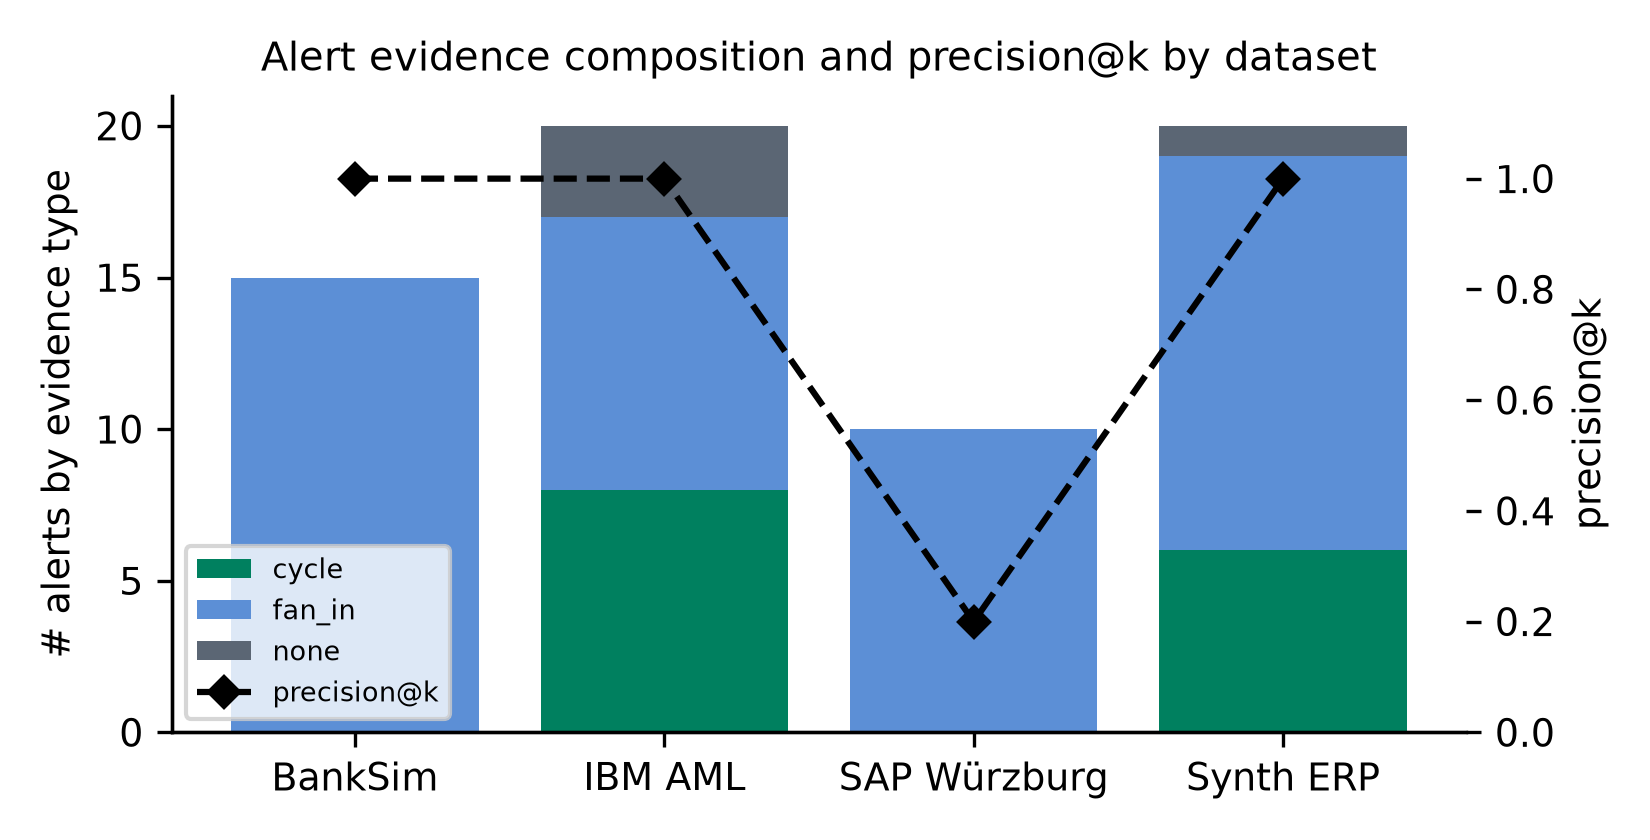
\includegraphics[width=\columnwidth]{figures/alert_evidence_mix.png}
\caption{Composition of graph evidence behind each dataset's top-$k$ alerts
(fan-in vs.\ cycle vs.\ no reconstructable structure), alongside precision@$k$.
Every bar sums to $k$ from Table~\ref{tab:alert_precision}.}
\label{fig:evidence_mix}
\end{figure}


\subsection{System: From Research Pipeline to Production Audit Console}\label{sec:system}\label{sec:production}

The preceding sections establish a narrow, defensible research claim about topology's marginal value under leakage-free evaluation. That claim is deliberately silent on whether the resulting models can run anywhere near a real ledger. Continuous-auditing research has long argued that a control is only as useful as the workflow that consumes it~\cite{vasarhelyi2012acceptance}, and post-implementation audits of ERP deployments routinely find that analytically sound models never reach production because the serving path, the data-integrity guarantees, and the operational evidence were never engineered~\cite{mamakou2024postimplementation}. This section describes what was actually built to close that gap: a Procure-to-Pay ERP core with a forensic audit console in front of it, an online scoring service that reuses the research pipeline's own feature-computation classes rather than reimplementing them, database-enforced financial-integrity invariants that do not trust application code to behave, and a measured (not assumed) performance and reliability profile. Every number in this section is either read directly from a project artifact file or drawn from a documented, reproducible test run; none are projected.

\subsubsection{Architecture Overview}\label{sec:system-arch}

The application is a conventional three-tier system chosen for auditability over novelty, consistent with the broader finding that ERP-adjacent ML systems succeed or fail on integration discipline more than on model sophistication~\cite{jawad2024erp}. A FastAPI backend exposes the ledger's domain objects (vendors, AP invoices, payments, payment runs, GL accounts, journal entries, audit alerts) through versioned REST routes (\texttt{app/api/\{vendors,invoices,payments,gl,alerts,auth,system\}.py}), backed by a normalized PostgreSQL schema and a Redis layer used for both response caching and idempotency-key bookkeeping. A React/TypeScript single-page frontend (\texttt{web/}) provides the clerk-facing ERP screens and the auditor-facing alert console. Neo4j sits alongside this stack strictly as a visualization and path-explanation surface for detected fraud alerts, never as a scoring dependency — the project's own methodology rules record that an earlier iteration let Neo4j silently become a load-bearing (and memory-exhausted) component of the scoring path, and this build deliberately keeps the database graph decorative.

The detail that distinguishes this system from a typical ML-in-the-loop web application is the scoring layer's relationship to the research code. \texttt{app.services.scoring\_service.FraudScoringService} does not reimplement the topology or tabular feature logic; it holds a live \texttt{OnlineTopologyState} and \texttt{OnlineOrdinaryState} per dataset/tenant, constructed directly from \texttt{topology.window\_graph.WindowGraph} and \texttt{topology.lap\_memory.LapMemory} — the exact classes \texttt{topology.engine.extract\_features} uses in the offline batch pipeline — plus a Welford-based incremental counterpart to the batch ordinary-feature builder. One instance is loaded per dataset at application startup from the persisted "online" bundle (\texttt{app/services/scoring\_registry.py}), and \texttt{/ready} reports honestly unavailable until at least one scoring service has loaded, rather than reporting healthy while silently unable to score. A single live ERP payment is routed to the \texttt{synth\_erp} scoring instance, the one dataset whose categorical vocabulary (\texttt{vendor\_payment}, \texttt{payroll}, \texttt{recurring\_bill}, \ldots) is a domain match for real AP postings.

%% FIGURE TODO: box-and-arrow diagram of the deployed system — ERP core (FastAPI + Postgres + Redis) on the left, the React audit console reading from it, the FraudScoringService holding live WindowGraph/LapMemory/Welford state on the right wired into the payment-posting path, Neo4j hanging off the alert console as visualization-only, and Prometheus/Grafana/Uptime Kuma scraping the API at the bottom — with a visual callout that the offline research pipeline (TGN training) is NOT in this runtime picture.
\begin{figure}[t]
  \centering
  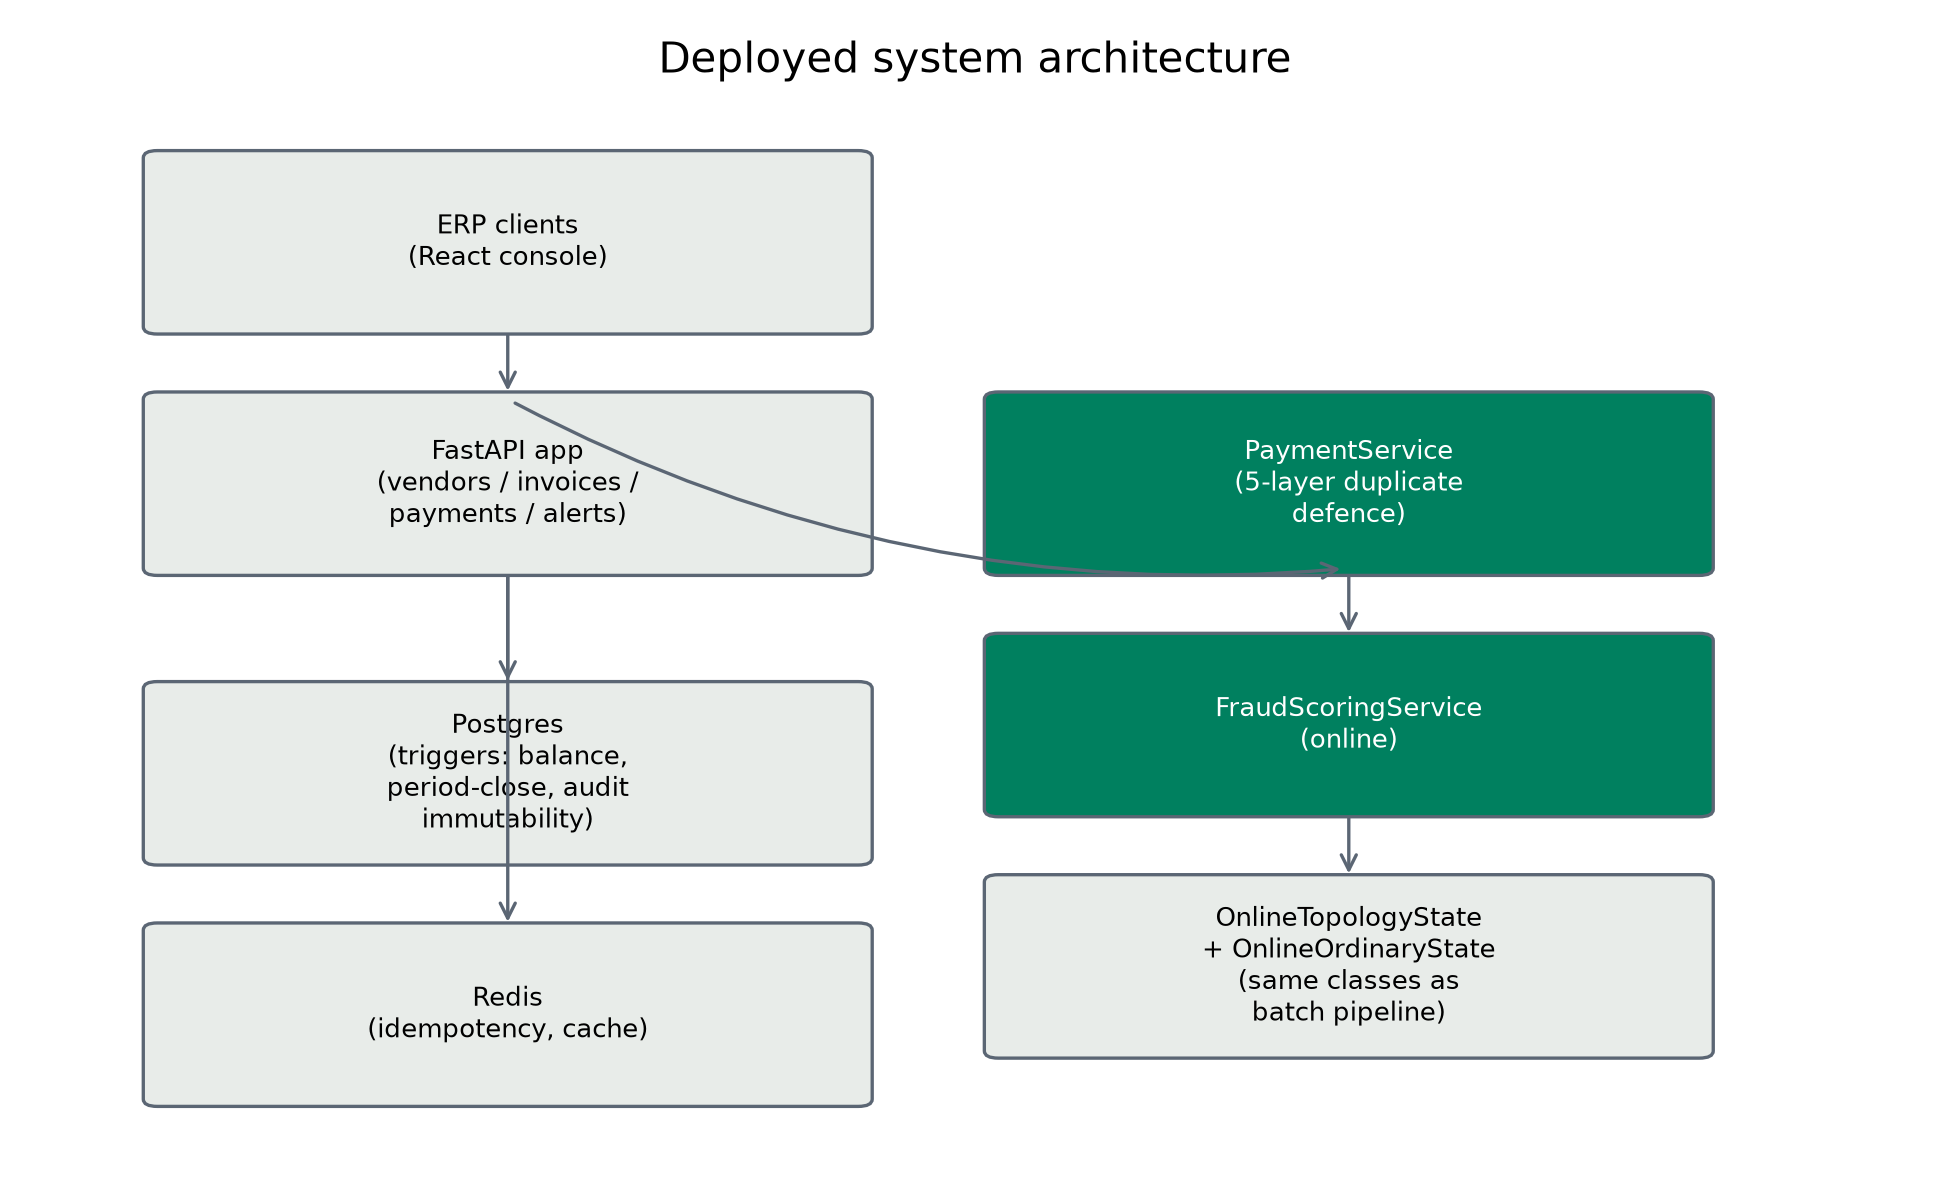
\includegraphics[width=\columnwidth]{figures/system_architecture.png}
  \caption{Deployed system architecture. The online \texttt{FraudScoringService} reuses the research pipeline's \texttt{WindowGraph}/\texttt{LapMemory} classes directly rather than a reimplementation; the offline TGN training path (Section~V) is not part of the serving runtime.}
  \label{fig:architecture}
\end{figure}

Correctness of the reuse, not merely its existence, is what makes the online path trustworthy: \texttt{tests/test\_online\_topology\_parity.py} replays 20{,}000 real transactions through both the batch \texttt{extract\_features} loop and \texttt{OnlineTopologyState.score\_transaction}, asserting every one of the thirteen topology feature columns matches exactly, row for row, with zero mismatches. The read-then-insert ordering inside the online class is copied line-for-line from the batch engine specifically to preserve this guarantee — the online driver differs only in holding one graph and two lap-memory instances alive across calls instead of discarding them after a single DataFrame pass.

\subsubsection{Financial Integrity as Database-Enforced Invariants}\label{sec:system-integrity}

An audit console is only as trustworthy as the ledger it reads from, and a recurring theme in ERP-integrity failures is that correctness logic lives entirely in application code that a bug, a bypassed service layer, or a future direct-SQL script can silently violate. This system treats three financial invariants as properties the database itself refuses to break, implemented as Postgres triggers (\texttt{alembic/versions/6192dae4f4a4\_gl\_invariants\_triggers.py}) rather than API-layer checks alone:

\begin{itemize}
  \item \textbf{Double-entry balance.} A \texttt{DEFERRABLE INITIALLY DEFERRED} constraint trigger on \texttt{journal\_lines} sums debits and credits per \texttt{journal\_entry\_id} and raises at \texttt{COMMIT}, not after each inserted line — necessary because a multi-line entry inserts its debit and credit rows separately and would fail a per-row check on every legitimate entry.
  \item \textbf{Period close.} An ordinary \texttt{BEFORE INSERT OR UPDATE} trigger on \texttt{journal\_entries} rejects any entry referencing a \texttt{fiscal\_period} whose status is not \texttt{open}. A FastAPI-level check exists purely to return a friendly \texttt{409} before the raw database exception would; the trigger is the actual enforcement.
  \item \textbf{Audit-log immutability.} \texttt{UPDATE} and \texttt{DELETE} on \texttt{audit\_log} are rejected outright by trigger, unconditionally. Only \texttt{INSERT} is a valid operation — the append-only property a SOX-style audit trail requires is a database guarantee here, not an application convention that a careless migration could quietly undermine.
\end{itemize}

Duplicate-payment prevention receives the same defense-in-depth treatment, layered so that no single control is trusted alone (\texttt{app/services/payment\_service.py}). An idempotency-key middleware replays the stored response for a retried request with the same key rather than re-executing it — the client-supplied-key pattern Helland~\cite{helland2012idempotence} argues is the only reliable way to make a mutating financial operation safe to retry, since the alternative (asking the caller never to retry, or de-duplicating on inferred request similarity) either fails under real network conditions or is not decidable in general. Independently, \texttt{create\_payment} takes a \texttt{SELECT ... FOR UPDATE} row lock on the target invoice \emph{before} checking for an existing active payment, closing the check-then-act race that two \emph{different} idempotency keys targeting the same invoice would otherwise open — the scenario a retry-only defense cannot cover, since it is two independent actors, not one repeated request. A partial unique index (\texttt{uq\_payments\_invoice\_live}, Module 3) is the database-level backstop if both application layers are ever bypassed. A \texttt{pg\_advisory\_xact\_lock} per vendor serializes an entire payment run, not just one invoice at a time. Finally, \texttt{tools/reconcile\_payments.py} is a periodic sweep that treats any invoice with more than one non-void payment as an incident — the tripwire for "we were wrong somewhere," not a preventive control. Table~\ref{tab:reliability} reports the formalized, automated test of this defense under real concurrency.

